\documentclass[aspectratio=169,10pt]{beamer}

\usepackage{luatexja}
\usepackage{luatexja-fontspec}
\setsansfont{Helvetica Neue}
\setsansjfont{Noto Sans JP}
\setmonofont{Menlo}

\usepackage{amsmath,amssymb,bm,mathtools}
\usepackage{booktabs,array,multirow}
\usepackage{graphicx}
\usepackage{tikz}
\usetikzlibrary{arrows.meta,positioning,calc,fit,shapes.geometric,decorations.pathreplacing}
\usepackage[backend=biber,style=authoryear-comp,maxcitenames=2,maxbibnames=99,doi=true,isbn=false,url=false,giveninits=true]{biblatex}
\addbibresource{capacity_mnar_references_mathdense.bib}

% ---------- Theme ----------
\usetheme{default}
\definecolor{Navy}{HTML}{183153}
\definecolor{Teal}{HTML}{0F6B6D}
\definecolor{Sky}{HTML}{EAF3F7}
\definecolor{Sand}{HTML}{F5F1E8}
\definecolor{Brick}{HTML}{A23B3B}
\definecolor{Green}{HTML}{2F6B4F}
\definecolor{GrayText}{HTML}{4E5968}
\definecolor{LightGray}{HTML}{F4F6F8}

\setbeamercolor{normal text}{fg=black,bg=white}
\setbeamercolor{structure}{fg=Navy}
\setbeamercolor{frametitle}{fg=white,bg=Navy}
\setbeamercolor{title}{fg=Navy}
\setbeamercolor{subtitle}{fg=Teal}
\setbeamercolor{block title}{fg=Navy,bg=Sky}
\setbeamercolor{block body}{fg=black,bg=Sky!45}
\setbeamercolor{alerted text}{fg=Brick}
\setbeamercolor{example text}{fg=Green}
\setbeamercolor{footline}{fg=GrayText,bg=white}

\setbeamertemplate{navigation symbols}{}
\setbeamertemplate{itemize item}{\color{Teal}$\blacktriangleright$}
\setbeamertemplate{itemize subitem}{\color{Navy}$\bullet$}
\setbeamertemplate{enumerate item}{\color{Navy}\insertenumlabel.}
\setbeamertemplate{blocks}[rounded][shadow=false]
\setbeamertemplate{bibliography item}{}
\setbeamertemplate{footline}{%
  \leavevmode%
  \hbox{%
    \begin{beamercolorbox}[wd=.84\paperwidth,ht=2.35ex,dp=1.0ex,leftskip=1.2em]{footline}%
      \scriptsize 欠測IVと潜在変数モデリングによる非無作為欠測の識別
    \end{beamercolorbox}%
    \begin{beamercolorbox}[wd=.16\paperwidth,ht=2.35ex,dp=1.0ex,rightskip=1.2em plus1fil]{footline}%
      \scriptsize \insertframenumber/\inserttotalframenumber
    \end{beamercolorbox}%
  }%
  \vskip0pt%
}

\setbeamerfont{title}{size=\LARGE,series=\bfseries}
\setbeamerfont{subtitle}{size=\large}
\setbeamerfont{author}{size=\normalsize}
\setbeamerfont{institute}{size=\small}
\setbeamerfont{frametitle}{size=\large,series=\bfseries}
\setbeamerfont{normal text}{size=\small}
\setbeamerfont{footnote}{size=\tiny}
\setlength{\leftmargini}{1.5em}
\setlength{\leftmarginii}{1.3em}
\setlength{\tabcolsep}{4pt}
\renewcommand{\arraystretch}{1.16}

% ---------- Commands ----------
\newcommand{\E}{\mathbb{E}}
\newcommand{\Prb}{\mathbb{P}}
\newcommand{\1}{\mathbf{1}}
\newcommand{\indep}{\mathrel{\perp\!\!\!\perp}}
\newcommand{\Y}{\bm{Y}}
\newcommand{\V}{\bm{V}}
\newcommand{\Z}{\bm{Z}}
\newcommand{\X}{\bm{X}}
\newcommand{\D}{\bm{D}}
\newcommand{\A}{\bm{A}}
\newcommand{\argmax}{\operatorname*{arg\,max}}
\newcommand{\Tail}{\operatorname{Tail}}
\newcommand{\Neutral}{\operatorname{Neutral}}
\newcommand{\Var}{\operatorname{Var}}
\newcommand{\Cov}{\operatorname{Cov}}
\newcommand{\supp}{\operatorname{supp}}
\newcommand{\rank}{\operatorname{rank}}
\newcommand{\Range}{\operatorname{Range}}
\newcommand{\ord}{\operatorname{ord}}
\newcommand{\Top}{\operatorname{Top}}
\newcommand{\Unif}{\operatorname{Unif}}
\newcommand{\dd}{\mathrm d}

\tikzset{
  box/.style={draw=Navy, rounded corners=2pt, minimum height=9mm, align=center, inner sep=4pt, font=\small, fill=white},
  softbox/.style={box, fill=Sky!60},
  sandbox/.style={box, fill=Sand!75},
  arr/.style={-{Latex[length=2.1mm,width=1.5mm]}, line width=.7pt, draw=Navy},
  darr/.style={arr,dashed,draw=GrayText},
  note/.style={font=\scriptsize,align=center,text=GrayText}
}

% ---------- Metadata ----------
\title{欠測IVと潜在変数モデリングによる\\非無作為欠測の識別}
\subtitle{多変量MNARのノンパラメトリック識別とオンラインレビューへの応用}
\author{本多 将大 \quad 星野 崇宏 \quad 大津 泰介}
\institute{慶應義塾大学・理化学研究所・London School of Economics and Political Science}
\date{日本統計学会研究報告}

\begin{document}

% REVIEW FIX 01: complete-case results are moved to the appendix.
% REVIEW FIX 02: observed data and structural support are defined explicitly.
% REVIEW FIX 03: the main positive result is target-specific representer identification.
% REVIEW FIX 04: identified targets are limited to supported marginals/functionals.
% REVIEW FIX 05: Model 1 conditions only on fully observed context.
% REVIEW FIX 06: crowd-out comparative statics no longer condition on the varied outcome.
% REVIEW FIX 07: capacity monotonicity uses the ranking variable, not noisy salience.
% REVIEW FIX 08: U-shaped tail inflation and J-shaped valence asymmetry are separated.
% REVIEW FIX 09: self-censoring comparisons include positivity and upward-closed support.
% REVIEW FIX 10: Model 2 is retained in the appendix as a partial-identification extension.
% REVIEW FIX 11: Model 3 is retained in the appendix as a weak-but-many extension.
% REVIEW FIX 12: latent measurement identification is stated with anchor conditions.
% REVIEW FIX 13: experiments evaluate mechanisms/recovery, not identification assumptions.
% REVIEW FIX 14: oracle, naive, and corrected estimators share one estimand.
% REVIEW FIX 15: algorithmic amplification is tested with randomized ranking.
% REVIEW RESPONSE 16: the selection equation is positioned as a generalized Roy model.
% REVIEW RESPONSE 17: target-specific representer identification is the main positive result.
% REVIEW RESPONSE 18: full-law identification and Models 2/3 are retained in the appendix.

% 1 ---------------------------------------------------------------------------
\begin{frame}[plain]
\begin{tikzpicture}[remember picture,overlay]
  \fill[Sky!55] (current page.north west) rectangle ([yshift=-1.45cm]current page.north east);
  \fill[Navy] ([yshift=0.55cm]current page.south west) rectangle (current page.south east);
  \draw[Teal,line width=2.2pt] ([xshift=1.05cm,yshift=-1.55cm]current page.north west) -- ([xshift=-1.05cm,yshift=-1.55cm]current page.north east);
\end{tikzpicture}
\vspace{1.5cm}
\titlepage
\end{frame}

% 2 ---------------------------------------------------------------------------
\begin{frame}[shrink=8]{Motivation：多変量MNARからマーケティング実証へ}
\begin{columns}[T,onlytextwidth]
\begin{column}{0.50\textwidth}
\begin{block}{マイクロデータの非観測問題}
\scriptsize
欠測値，選択，反実仮想の非観測は頻繁に生じる。MNARでは未観測値自身が観測確率を動かすため，
\[
\Prb(D=1\mid Y,X)\text{ depends on }Y
\quad\Rightarrow\quad
f(Y\mid D=1,X)\ne f(Y\mid X).
\]
観測集団だけに基づく推論は一般に偏る。
\end{block}
\begin{block}{欠測IVによるノンパラメトリック識別}
\scriptsize
選択だけを動かす通常のIVでは，アウトカム分布全体の点識別は困難である。一方，\textcite{dHaultfoeuille2010} は
\[
D\indep V\mid Y,X,
\qquad V\not\indep Y\mid X
\]
と完備性の下で，欠測アウトカムの分布を関数形なしに識別した。近年は自己値依存・他項目依存の多変量MNARについても識別・推定が示されている
\parencite{LiMiaoShpitserTchetgen2023,MalinskyShpitserTchetgen2022}。
\end{block}
\end{column}
\begin{column}{0.47\textwidth}
\begin{alertblock}{オンラインレビューは制約付き多変量MNARである}
\scriptsize
レビュー投稿は自己選択的で，極端な経験を選ぶpolarity self-selectionにより，公開評価はJ字型またはpolarな分布になる
\parencite{SchoenmuellerNetzerStahl2020,HuPavlouZhang2017}。

\medskip
個人 $i$ は $m$ 個の私的評価を持つが，認知的・行動的な投稿コストにより公開できるのは $K_i<m$ 件である。
\[
\Y_i=(Y_{i1},\ldots,Y_{im})',
\qquad
\sum_{j=1}^{m}D_{ij}=K_i.
\]
このとき多数の潜在的レビューが有限の開示枠を競い，$D_{ij}$ は自己値 $Y_{ij}$ と他項目 $\Y_{i,-j}$ の双方に依存する。
\end{alertblock}
\begin{block}{中心的な問い}
\scriptsize
構造的ゼロとcross-item crowd-outをもつ分布から，平均評価や極端評価率をどこまでノンパラメトリックに回復できるか。
\end{block}
\end{column}
\end{columns}
\end{frame}

% 3 ---------------------------------------------------------------------------
\begin{frame}[shrink=7]{多変量MNARでは，項目 $j$ の公開が評価ベクトル全体に依存する}
\begin{columns}[T,onlytextwidth]
\begin{column}{0.57\textwidth}
\centering
\begin{tikzpicture}[x=1.28cm,y=1.05cm,scale=.84,transform shape]
  \node[softbox,minimum width=1.55cm] (dj) at (0,3.8) {$D_{ij}$};
  \node[softbox,minimum width=1.75cm] (dm) at (4.2,3.8) {$\D_{i,-j}$};
  \node[box,minimum width=1.55cm] (yj) at (0,1.85) {$Y_{ij}$};
  \node[box,minimum width=1.75cm] (ym) at (4.2,1.85) {$\Y_{i,-j}$};
  \node[sandbox,minimum width=1.55cm] (vj) at (0,0) {$V_{ij}$};
  \node[sandbox,minimum width=1.75cm] (vm) at (4.2,0) {$\V_{i,-j}$};
  \node[box,minimum width=1.5cm] (xk) at (-2.25,1.85) {$\X_i,K_i$};

  \draw[arr,draw=Teal] (vj) -- (yj);
  \draw[arr,draw=Teal] (vm) -- (ym);
  \draw[arr] (xk) -- (yj);
  \draw[arr] (xk) to[bend left=18] (dj);
  \draw[arr,draw=Brick,line width=1.0pt] (yj) -- (dj);
  \draw[arr,draw=Brick,line width=1.0pt] (ym) -- (dm);
  \draw[arr,draw=Brick,dashed] (ym) to[bend right=17] (dj);
  \draw[arr,draw=Brick,dashed] (yj) to[bend left=17] (dm);
  \draw[<->,draw=GrayText,line width=.7pt] (yj) -- node[above,font=\scriptsize]{相互依存} (ym);
  \draw[decorate,decoration={brace,amplitude=5pt},draw=Navy]
    (-.75,4.45) -- (4.95,4.45)
    node[midway,above=6pt,font=\scriptsize] {$\sum_{\ell=1}^{m}D_{i\ell}=K_i$};

  \node[note,text=Brick] at (2.1,3.15) {実線：自己値依存\quad{}破線：cross-item crowd-out};
  \node[note,text=Teal] at (2.1,-.65) {$V$は常時観測されるshadow signal};
\end{tikzpicture}
{\scriptsize
\[
Y_{ij}^{\mathrm{obs}}=D_{ij}Y_{ij},
\qquad
O_i=(\X_i,K_i,\V_i,\D_i,\Y_i^{\mathrm{obs}}).
\]}
\end{column}
\begin{column}{0.40\textwidth}
\begin{block}{既存の二つのcensoring関係}
\scriptsize
\textbf{Self-censoring:}
\[
D_{ij}\indep\Y_{i,-j}
\mid \X_i,Y_{ij},\D_{i,-j}.
\]
\textbf{No self-censoring:}
\[
D_{ij}\indep Y_{ij}
\mid \X_i,\Y_{i,-j},\D_{i,-j}.
\]
\end{block}
\begin{alertblock}{容量制約付き選択}
\scriptsize
\[
\Prb(D_{ij}=1\mid\Y_i,\X_i,K_i)
\]
は $Y_{ij}$ と $\Y_{i,-j}$ の双方に依存する。したがって既存のどちらのcensoring独立性にも一般に属さない。
\end{alertblock}
\begin{block}{Shadow-variable route}
\tiny
$C_{ij}=(\X_i,K_i,\V_{i,-j})$ を常時観測文脈とし，
\[
D_{ij}\indep V_{ij}\mid Y_{ij},C_{ij},
\qquad
V_{ij}\not\indep Y_{ij}\mid C_{ij}
\]
とtarget-specific bridgeにより，平均・裾確率を直接回復する。
\end{block}
\end{column}
\end{columns}
\end{frame}

% 4 ---------------------------------------------------------------------------
\begin{frame}[shrink=5]{本研究は方法論を実験で検証し，プラットフォーム増幅へ拡張する}
\begin{columns}[T,onlytextwidth]
\begin{column}{0.32\textwidth}
\begin{block}{1. 方法論}
\scriptsize
容量制約付きmultiple selectionを，構造的ゼロと項目間依存をもつ多変量MNARとして定式化する。既存モデルと識別仮定が異なるため，平均・裾確率のtarget-specific bridgeによるノンパラメトリック識別を与える。
\end{block}
\end{column}
\begin{column}{0.32\textwidth}
\begin{block}{2. 実験1}
\scriptsize
同一標本から全項目の私的評価（oracle）と公開評価（public）を取得する。開示容量 $K_i$ をランダム化し，MNARのcrowd-outと識別・回復性能を直接比較する。
\end{block}
\end{column}
\begin{column}{0.32\textwidth}
\begin{block}{3. 実験2}
\scriptsize
発展的に，実際の擬似プラットフォームでrandom，helpfulness，生成AIランキングを比較し，投稿段階の歪みが表示アルゴリズムによって増幅されるかを検証する。
\end{block}
\end{column}
\end{columns}
\begin{alertblock}{期待される成果とアウトリーチ}
\scriptsize
観察される公開評価から母集団の評価汎関数を回復する理論と実証を得る。統計学，情報理論，経済学，商学，心理学，機械学習を横断し，SNS，口コミ，体験談，苦情投稿などの投稿コストと取得データが社会的評価分布に与える影響を明らかにする。
\end{alertblock}
\end{frame}

% 5 ---------------------------------------------------------------------------
\begin{frame}[shrink=5]{既知なのは極端性，未解明なのは経験間の競争である}
\begin{columns}[T,onlytextwidth]
\begin{column}{0.42\textwidth}
\begin{block}{先行研究が示したこと}
\scriptsize
\begin{itemize}
\item 低頻度レビュアーほど1・5星が過剰になる。
\item self-selected review は forced review より極端になる。
\item acquisition bias と underreporting bias により公開分布は母集団を代表しない。
\end{itemize}
\end{block}
\centering

\includegraphics[width=0.97\linewidth,height=0.29\textheight,keepaspectratio]{review_polarity_yelp_fig3.png}
\end{column}
\begin{column}{0.56\textwidth}
\centering

\includegraphics[width=0.72\linewidth,height=0.36\textheight,keepaspectratio]{review_capacity_selection_example.png}
\begin{alertblock}{本研究が追加する比較}
\scriptsize
\[
K_i\downarrow
\ \Longrightarrow\ 
\text{高salience経験への集中}
\ \Longrightarrow\ 
\text{cross-item crowd-out}.
\]
$Y_{ij}$ を固定しても，他項目により強い経験があると $j$ は公開枠から押し出される。
この依存構造と $K_i$ の因果効果を明示的に検証する。
\end{alertblock}
{\tiny Source of left figure: \textcite{SchoenmuellerNetzerStahl2020}, Figure 3.}
\end{column}
\end{columns}
\end{frame}

% 6 ---------------------------------------------------------------------------
\begin{frame}[shrink=7]{Strategic sample selection を欠測パターンへ写像する}
\begin{columns}[T,onlytextwidth]
\begin{column}{0.45\textwidth}
\begin{block}{既存の selected experiment}
\scriptsize
候補 $k$ 個から上位 $n$ 個を観測する
\parencite{DiTillioOttavianiSorensen2021}。
\[
X_1\ge\cdots\ge X_n
=\text{top }n\text{ of }k>n.
\]
最大値の分布は
\[
G_1(x\mid\theta)=F^k(x\mid\theta)
\]
となり，ランダム標本とは異なる。
\end{block}
\begin{alertblock}{レビューへの読み替え}
\scriptsize
\[
\underbrace{k}_{\text{presample}}
\leftrightarrow
\underbrace{m}_{\text{経験数}},
\qquad
\underbrace{n}_{\text{sample}}
\leftrightarrow
\underbrace{K_i}_{\text{公開枠}}.
\]
\end{alertblock}
\end{column}
\begin{column}{0.53\textwidth}
\centering

\includegraphics[width=\linewidth,height=0.43\textheight,keepaspectratio]{strategic_sample_selection_fig1.jpg}
\begin{block}{本研究の統計的写像}
\scriptsize
\[
\D_i=r_{K_i}\{\A_i(\Y_i,\X_i,\varepsilon_i)\},
\qquad
Y_{ij}^{obs}=D_{ij}Y_{ij}.
\]
経済的な選択集合を，多変量欠測パターン $\D_i$ として扱う。
\end{block}
{\tiny Source: \textcite{DiTillioOttavianiSorensen2021}, Figure 1.}
\end{column}
\end{columns}
\end{frame}

% 7 ---------------------------------------------------------------------------
\begin{frame}{選択方程式はgeneralized Roy modelに含まれる}
\begin{columns}[T,onlytextwidth]
\begin{column}{0.49\textwidth}
\begin{block}{包含関係}
\scriptsize
各レビュー候補には公開効用 $A_{ij}$ があり，個人は容量 $K_i$ の下で
\[
S_i(K_i)\in\argmax_{|S|\le K_i}\sum_{j\in S}A_{ij}
\]
を選ぶ。これは非金銭的効用と複数選択を許す
\textbf{capacity-constrained generalized Roy model} と読める。
\end{block}
\begin{alertblock}{新規性を主張しない部分}
\scriptsize
\textcite{dHaultfoeuille2010} はshadow IVを
unobserved-sector Roy modelへ適用できることを既に示している。
したがって「Roy modelへのshadow-variable法の適用」自体は本研究の新規性ではない。
\end{alertblock}
\end{column}
\begin{column}{0.48\textwidth}
\begin{block}{本研究が検証する部分}
\scriptsize
\begin{enumerate}
\item exact top-$K$ による構造的ゼロ；
\item 他項目との競争によるcross-item crowd-out；
\item oracleとpublicを同一標本から得る回復性能；
\item $K_i$ とランキングのランダム化による因果比較。
\end{enumerate}
\end{block}
\begin{alertblock}{位置づけ}
\scriptsize
方法論の中心は新しいRoy識別定理ではなく，
容量制約付きレビューをdependent multivariate MNARとして実装し，
選択機構とshadow補正を直接評価することである。
\end{alertblock}
\end{column}
\end{columns}
\end{frame}

% 8 ---------------------------------------------------------------------------
\begin{frame}[shrink=5]{既存の多変量MNARは top-$K$ の支持集合と両立しない}
\scriptsize
\begin{tabular}{>{\raggedright\arraybackslash}p{0.18\textwidth}
                >{\raggedright\arraybackslash}p{0.37\textwidth}
                >{\raggedright\arraybackslash}p{0.36\textwidth}}
\toprule
モデル & 識別仮定 & top-$K$ との相違 \\
\midrule
\textbf{Self-censoring}
&
$D_j\indep Y_{-j}\mid X,Y_j,D_{-j}$。
加えて各 supported pattern の positivity と，
$d\le d'$ なら $d'$ も supported という upward closure を置く。
&
$\sum_jD_j=K<m$ では上位パターン，特に $\bm1_m$ が存在せず，
upward closure が破れる。
\\
\addlinespace
\textbf{No self-censoring}
&
$D_j\indep Y_j\mid X,Y_{-j},D_{-j}$ と
$\Prb(\D=\bm1_m\mid\Y,X)>\sigma$。
&
自己値が公開を動かす極端性選択を排除し，完全ケース positivity も破れる。
\\
\addlinespace
\textbf{Complete-case missing IV}
&
$R^{cc}\indep V\mid\Y,X$，
$\Prb(R^{cc}=1\mid\Y,X)>0$。
&
$R^{cc}=\1\{\D=\bm1_m\}=0$ a.s. で，識別モーメント自体が消える。
\\
\addlinespace
\textbf{本研究}
&
項目・supported blockごとにshadow conditionと
target-specific representer bridgeを置く。
&
平均・裾確率を直接回復する。分布全体の識別には追加の完備性を要する。
\\
\bottomrule
\end{tabular}
\vspace{1mm}
{\tiny Sources: \textcite{LiMiaoShpitserTchetgen2023,MalinskyShpitserTchetgen2022,dHaultfoeuille2010}.}
\end{frame}

% 6 ---------------------------------------------------------------------------
\begin{frame}{公開効用は positive WOM と negative WOM の二経路をもつ}
個人 $i$ の財 $j$ に対する公開動機を
\[
M^+_{ij}=f_+\bigl((Y_{ij}-c_0)_+,\Y_{i,-j},\X_i\bigr),
\qquad
M^-_{ij}=f_-\bigl((c_0-Y_{ij})_+,\Y_{i,-j},\X_i\bigr)
\]
とする。$M^+$ は self-enhancement・他者支援・企業支援，
$M^-$ は negative feelings の解放・他者への警告を含む
\parencite{HennigThurauEtAl2004,Berger2014}。
\[
A_{ij}
=a_+(M^+_{ij})+a_-(M^-_{ij})-\kappa_{ij}+\varepsilon_{ij},
\qquad a_+',a_-',f_+',f_-'\ge0.
\tag{U}
\]
\begin{block}{評価から公開効用への単調経路}
$Y_{ij}>c_0$ では positive WOM，$Y_{ij}<c_0$ では negative WOM が公開効用を高め得る。
したがって極端性は公開効用を高めるが，正負の傾きは等しい必要がない。
\end{block}
\end{frame}

% 7 ---------------------------------------------------------------------------
\begin{frame}{容量制約が公開集合を決める}
開示集合は
\[
S_i(B_i)\in\argmax_{S\subseteq\{1,\ldots,m\}}
\sum_{j\in S}A_{ij}
\quad\text{s.t.}\quad
\sum_{j\in S}c_{ij}\le B_i,
\qquad D_{ij}=\1\{j\in S_i(B_i)\}.
\tag{SEL}
\]
\begin{block}{Top-$K$ 特殊ケース}
$c_{ij}=1$，$B_i=K_i$，同順位なし，かつ正確に $K_i$ 件を選ぶなら
\[
D_{ij}=\1\{A_{ij}\ge A_{i,(K_i)}\},
\]
ただし $A_{i,(K_i)}$ は降順 $K_i$ 番目の公開効用である。
\end{block}
\end{frame}

% 8 ---------------------------------------------------------------------------
\begin{frame}{命題1：Top-$K$ は自己単調性とcrowd-outを生む}
\begin{block}{命題1（自己単調性と競合経験効果）}
同順位がない exact top-$K$ 選択を考える。他の効用を固定すると
\[
A_{ij}\uparrow\quad\Longrightarrow\quad D_{ij}\ \text{は弱く増加する}.
\]
一方，$A_{ij}$ と $\A_{i,-\{j,\ell\}}$ を固定すると
\[
A_{i\ell}\uparrow\quad(\ell\ne j)
\quad\Longrightarrow\quad
D_{ij}\ \text{は弱く減少する}.
\tag{CO}
\]
\end{block}
\begin{alertblock}{識別可能な比較静学}
自己効用 $A_{ij}$ を固定しても，競合する $A_{i\ell}$ が上がれば
$j$ の公開確率は弱く下がる。これは itemwise 独立選択にはない
\textbf{experience-level crowd-out} である。
\end{alertblock}
\end{frame}

% 9 ---------------------------------------------------------------------------
\begin{frame}{命題2：公開容量が小さいほど選択効用は高くなる}
\begin{block}{命題2（容量比較静学）}
$A_{i(1)}\ge\cdots\ge A_{i(m)}$ とし
\[
\bar A_i(K)=K^{-1}\sum_{r=1}^{K}A_{i(r)}
\]
と置く。$K_1<K_2$ なら
\[
\bar A_i(K_1)\ge\bar A_i(K_2).
\tag{CAP}
\]
salience $s_{ij}$ について同じ結論を得るには
\[
\ord\{A_{ij}\}_{j=1}^m=\ord\{s_{ij}\}_{j=1}^m\quad\text{a.s.}
\]
が必要である。単に $A_{ij}=v(s_{ij})+\varepsilon_{ij}$ と置くだけでは順位一致は従わない。
\end{block}
\end{frame}

% 10 --------------------------------------------------------------------------
\begin{frame}[shrink=7]{実験仮説：U字型の裾過剰とJ字型の非対称を区別する}
評価の方向別salienceを
\[
s(y)=\alpha_+(y-c_0)_++\alpha_-(c_0-y)_+,
\qquad \alpha_+,\alpha_-\ge0
\]
とする。
\begin{columns}[T,onlytextwidth]
\begin{column}{0.48\textwidth}
\begin{block}{U字型を導く追加条件}
\[
\alpha_+=\alpha_->0
\]
に加え，公開効用の順位が極端性順位と整合し，選択が非退化なら，容量制約は両側の裾を過剰にする。
\[
\Prb(|Y-c_0|\ge t\mid D=1)
\ge
\Prb(|Y-c_0|\ge t).
\]
この順位整合性はRoy構造だけからは従わず，実験仮説として検証する。
\end{block}
\end{column}
\begin{column}{0.48\textwidth}
\begin{alertblock}{J字型には非対称性が必要}
\[
\alpha_+>\alpha_-
\]
または母分布の正側への非対称性があると，5星側が1星側より強く残る。
\[
\Prb(Y=5\mid D=1)-\Prb(Y=1\mid D=1)
\]
は別の対象であり，極端性だけからJ字型とは結論できない。
\end{alertblock}
\end{column}
\end{columns}
\end{frame}

% 9 ---------------------------------------------------------------------------
\begin{frame}{観測データは完全ケースを含まない pattern data である}
理論では共通の $m$ 項目を考える。$K_i\in\{1,\ldots,m-1\}$ とし，
\[
\mathcal D_{m,K_i}
=\left\{d\in\{0,1\}^m:\sum_{j=1}^m d_j=K_i\right\}.
\]
観測データは
\[
O_i=\left(\X_i,\V_i,K_i,\D_i,\Y_{i,\D_i}\right),
\qquad
\Y_{i,\D_i}=\{Y_{ij}:D_{ij}=1\}.
\tag{O}
\]
\begin{alertblock}{構造的ゼロ}
exact top-$K<m$ では $\Prb(\D_i=\bm1_m)=0$ であり，完全ケースは観測支持に含まれない。
\end{alertblock}
\end{frame}

\begin{frame}{Supported block が観測可能な同時分布を定める}
\begin{block}{Supported block}
$S\subseteq\{1,\ldots,m\}$ に対し
\[
R_{iS}=\prod_{j\in S}D_{ij},
\qquad
\Y_{iS}=(Y_{ij}:j\in S)',
\qquad
\mathcal C_{iS}=(\X_i,K_i,\V_{i,-S}).
\]
$S$ は
\[
\Prb(R_{iS}=1\mid\mathcal C_{iS})>0
\]
を満たすとき supported と呼ぶ。exact top-$K$ では $|S|\le K_i$ が必要である。
\end{block}
\begin{alertblock}{ポイント}
$R_{iS}$ は「$S$ の全成分が同時に観測されたか」を表す。
したがって各 block はスカラーの観測指標を持ち，欠測IVの条件付きモーメントを定義できる。
\end{alertblock}
\end{frame}

\begin{frame}{識別対象は支持される周辺分布と汎関数である}
\begin{block}{観測可能な支持}
集合 $S$ が supported なら，$R_{iS}=1$ の観測で $\Y_{iS}$ が同時に現れる。
一方，$|S|>K_i$ のブロックは構造的に観測されない。
\end{block}
\begin{alertblock}{識別対象}
主対象は $\E h(Y_{ij})$，$\Prb(Y_{ij}\in\{1,5\})$。
$K\ge2$ なら supported pair の共分散も対象になる。
full joint law $P(\Y)$ は追加構造なしには対象にしない。
\end{alertblock}
\[
\underbrace{|S|\le K}_{\text{observational support}}
\Rightarrow\text{candidate for recovery},
\qquad
|S|>K\Rightarrow\text{not observed jointly}.
\]
\end{frame}

% 10 --------------------------------------------------------------------------
\begin{frame}{定理1：完全ケース法は構造的ゼロにより適用できない}
\begin{block}{定理1（構造的ゼロ下の非識別）}
$K<m$ a.s. なら
\[
R^{cc}=\1\{\D=\bm1_m\}=0\quad\text{a.s.}
\]
したがって complete-case moment
\[
\E\left\{\frac{R^{cc}}{q(\Y,\X)}\middle|\V,\X\right\}=1
\]
を満たす $q$ は存在せず，complete-case missing-IV 定理は適用できない。
\end{block}
\begin{alertblock}{含意}
完全ケースの欠如は有限標本問題ではない。
$R^{cc}=0$ がデータ生成過程に組み込まれているため，完全ケースを用いる条件付きモーメントは定義できない。
\end{alertblock}
\end{frame}

\begin{frame}{定理1：supported block を超える結合分布は非識別である}
\begin{alertblock}{反例：$m=2,K=1$}
$\Prb(\D=(1,0))=\Prb(\D=(0,1))=1/2$，$\D\indep\Y$ とする。
\[
P_A:\ Y_1,Y_2\stackrel{i.i.d.}{\sim}\operatorname{Bernoulli}(1/2),
\]
\[
P_B:\ Y_1=Y_2\sim\operatorname{Bernoulli}(1/2).
\]
$P_A$ と $P_B$ は同じ観測データ法則 $P_O$ を生成するが，
\[
\Cov_A(Y_1,Y_2)=0,
\qquad
\Cov_B(Y_1,Y_2)=1/4.
\]
よって full joint law は非識別である。
\end{alertblock}
\begin{block}{識別境界}
観測データが同じでも未観測の依存構造は異なり得る。
追加構造なしに回復できる対象は supported block の法則に限定される。
\end{block}
\end{frame}

% 11 --------------------------------------------------------------------------
\begin{frame}{本文の識別対象は平均・裾確率である}
項目 $j$ について
\[
R_{ij}=D_{ij},\qquad
C_{ij}=(\X_i,K_i,\V_{i,-j}),\qquad
V_{ij}=Z^{pre}_{ij}
\]
とする。$C_{ij}$ と $V_{ij}$ は全員について観測される。
\begin{block}{Target-specific functionals}
\scriptsize
\[
\theta_{j,\tau}=\E\{\tau(Y_{ij},C_{ij})\},
\]
\[
\tau_{mean}(y,c)=y,\qquad
\tau_{tail}(y,c)=\1\{y\in\{1,5\}\},\qquad
\tau_{ext}(y,c)=|y-c_0|.
\]
\end{block}
\begin{alertblock}{識別方針}
full-data lawを先に識別するのではなく，実験で比較する平均・裾確率を直接識別する。
これにより，分布全体に必要な完備性より弱い条件を利用できる。
\end{alertblock}
\end{frame}

\begin{frame}{Target-specific representer bridgeを明示する}
\begin{block}{仮定 R1--R3}
\scriptsize
\[
\text{R1: }0<\Prb(R_{ij}=1\mid Y_{ij},C_{ij})\quad\text{a.s.}
\]
\[
\text{R2: }R_{ij}\indep V_{ij}\mid Y_{ij},C_{ij}.
\tag{SV}
\]
$\delta_{j,\tau}\in L^2(V_{ij},C_{ij})$ が存在して
\[
\text{R3: }\E\{\delta_{j,\tau}(V_{ij},C_{ij})
\mid R_{ij}=1,Y_{ij},C_{ij}\}
=\tau(Y_{ij},C_{ij}).
\tag{Bridge}
\]
\end{block}
\begin{alertblock}{作用素による表現}
\scriptsize
\[
(T_j^*\delta)(y,c)
=\E\{\delta(V_{ij},c)\mid R_{ij}=1,Y_{ij}=y,C_{ij}=c\}.
\]
bridge条件は $\tau\in\Range(T_j^*)$ である。解の存在は必要だが，一意性は要求しない
\parencite{LiMiaoTchetgen2023}。
これは対象識別の便利な十分条件であり，一般的な必要十分条件とは主張しない。
R1が成立しない場合は，対象をitemwise overlap populationへ限定する。
\end{alertblock}
\end{frame}

\begin{frame}{定理2：対象汎関数はfull lawなしに識別できる}
\begin{alertblock}{定理2（target-specific nonparametric identification）}
R1--R3 の下で
\[
\boxed{
\theta_{j,\tau}
=\E\left[
R_{ij}\tau(Y_{ij},C_{ij})
+(1-R_{ij})\delta_{j,\tau}(V_{ij},C_{ij})
\right].}
\tag{TF}
\]
右辺は観測データのみの汎関数であるため，$\theta_{j,\tau}$ は
ノンパラメトリックに識別される。
\end{alertblock}
\begin{block}{なぜ成立するか}
\scriptsize
R2により $V_{ij}\mid(Y_{ij},C_{ij})$ の分布は $R_{ij}$ に依存しない。
したがってR3は非公開者にも同じ条件付き平均を与え，
\[
\E\{(1-R_{ij})\delta_{j,\tau}\}
=\E\{(1-R_{ij})\tau(Y_{ij},C_{ij})\}.
\]
公開部分を加えると (TF) が従う。
\end{block}
\end{frame}

\begin{frame}{5段階評価ではbridge存在条件をrankで確認できる}
$Y_{ij}\in\{1,2,3,4,5\}$ とし，$V_{ij}$ も有限サポートをもつとする。
\[
H_j(c)=\left[
\Prb(V_{ij}=v\mid R_{ij}=1,Y_{ij}=y,C_{ij}=c)
\right]_{y,v}.
\]
\begin{block}{Target-specific condition}
\scriptsize
$\bm\tau_j(c)=(\tau(1,c),\ldots,\tau(5,c))'$ とするとbridge equationは
\[
H_j(c)\bm\delta_{j,\tau}(c)=\bm\tau_j(c).
\]
したがって必要なのは
\[
\bm\tau_j(c)\in\Range\{H_j(c)\}\quad\text{a.e. }c.
\tag{RC}
\]
\end{block}
\begin{alertblock}{完備性との違い}
\scriptsize
$\rank H_j(c)=5$ は全ての $\tau$ に対する十分条件だが，平均や裾確率には (RC) だけでよい。
これはfull-law識別の完備性より弱い。
\end{alertblock}
\end{frame}

% 12 --------------------------------------------------------------------------
\begin{frame}[shrink=6]{Model 1：top-$K$ の下ではshadow exclusionを追加仮定する}
選択写像を
\[
R_{ij}=r_j(\Y_i,\X_i,K_i,\bm\kappa_i,\bm\varepsilon_i^D)
\]
と書く。top-$K$ では $R_{ij}$ が $\Y_{i,-j}$ に依存するため，
(SV) はRoy構造だけから自動的には従わない。
\begin{alertblock}{原始的な十分条件の一例}
\scriptsize
\[
V_{ij}\indep
(\Y_{i,-j},\bm\varepsilon_i^D,\bm\kappa_i)
\mid Y_{ij},C_{ij},
\tag{P-SV}
\]
かつ $V_{ij}$ は $Y_{ij},C_{ij}$ を固定した後に公開効用 $A_{ij}$ へ直接入らない。
このとき未観測の競合評価と選択ショックを周辺化した後も
\[
R_{ij}\indep V_{ij}\mid Y_{ij},C_{ij}
\]
が保たれる。
\end{alertblock}
\begin{block}{限定}
\scriptsize
(P-SV) は強い維持仮定であり，実験だけでは証明できない。
二波測定・時点付きログ・複数信号・排除制約違反への感度分析で妥当性を補強する。
事前期待は期待不一致を通じて公開効用へ直接入り得るため，時間的先行だけでは十分でない。
\end{block}
\end{frame}

% 15 --------------------------------------------------------------------------
\begin{frame}{発展：潜在変数はsupported blocksを結ぶ追加構造である}
\begin{block}{測定モデル}
\scriptsize
\[
F_i=g(V_i,\X_i)+U_i,
\qquad
Y_{ij}=h_j(F_i,\X_i)+\varepsilon_{ij},
\]
\[
\E(U_i\mid V_i,\X_i)=0,
\qquad
\E(\varepsilon_{ij}\mid F_i,\X_i)=0.
\]
\end{block}
\begin{alertblock}{定理3の十分条件}
次を仮定する。
\begin{enumerate}
\item $K\ge3$ の層で三つの anchor items $a,b,c$ が jointly supported であり，付録Eの強い完備性条件により $P(Y_a,Y_b,Y_c,V,X)$ が識別される。
\item $Y_a,Y_b,Y_c$ は $(F,X)$ を条件に独立で，対応する条件付き期待値作用素が injective である。
\item $F$ の位置・尺度を正規化する。
\item 各 $j$ について $\{j,a,b\}$ が jointly supported で，同じ injectivity 条件を満たす。
\end{enumerate}
\end{alertblock}
\end{frame}

\begin{frame}{定理3：測定モデルはsupported blocksを接続する}
\begin{alertblock}{定理3（latent measurement extension）}
このとき三測定識別の議論 \parencite{HuSchennach2008} により，
$P(F\mid V,X)$ と測定kernel $P(Y_j\mid F,X)$ が正規化の下で識別される。
さらに
\[
g(v,x)=\E(F\mid V=v,X=x),
\qquad
h_j(f,x)=\E(Y_j\mid F=f,X=x)
\]
が識別される。
\end{alertblock}
\begin{block}{境界}
低ランク構造だけでは vector completeness は従わない。
定理3には supported anchors，measurement injectivity，正規化が必要である。
これは本文の実験的貢献に必要な仮定ではなく，full-law回復を目指す発展結果である。
\end{block}
\end{frame}

% 16 --------------------------------------------------------------------------
\begin{frame}{実験1：oracleとpublicを同一標本から取得する}
\begin{enumerate}
\item 共通候補30--40サービスから，少なくとも $J\simeq10$ の利用経験を持つ参加者をscreeningする。
\item private rating $Y_{ij}$，利用頻度・期間，課金，属性を取得して回答をlockする。
\item confirmatory analysis では
\[
K_i\in\{1,3\},\qquad \text{forced random-3}
\]
へランダム割当する。必要に応じ $K=5,10$ を補助群とする。
\item self-selected群は指定件数だけ公開対象を選び，選択した対象だけ短い自由記述を書く。基本報酬は評価方向と公開対象に依存させない。
\item 標本数は $n>100$ の固定値ではなく，個人内相関と三群比較を含む事前の検出力計算で決定する。
\end{enumerate}
\end{frame}

\begin{frame}{実験1：shadow測定時点と検証範囲を分ける}
\begin{alertblock}{Shadow signal の測定時点}
回顧的な利用前期待は recall bias により R2 の valid shadow と自動的にはみなさない。
target-specific point identificationを主張するconfirmatory studyでは，二波設計またはログにより
$V_{ij}^{pre}$ を評価形成前に測る。必要なら倫理審査を変更する。
\end{alertblock}
\begin{block}{実験が検証できる範囲}
実験は capacity effect，crowd-out，oracleに対する補正性能を評価する。
shadow exclusionやbridgeの存在そのものをデータだけで証明するものではない。
\end{block}
\begin{alertblock}{必要な設計変更}
R1--R3をconfirmatory claimにする場合は，倫理審査変更後の二波測定または
時点付きプラットフォームログを用いる。現行の回顧測定だけなら，付録の単調性boundsと感度分析を併記する。
\end{alertblock}
\end{frame}

% 17 --------------------------------------------------------------------------
\begin{frame}{Oracleとnaiveを同じperson-average targetで比較する}
person-average targetを
\[
\theta_h=\E\left\{\frac1m\sum_{j=1}^{m}h(Y_{ij})\right\}
\]
と固定する。完全データによるoracleは
\[
\widehat\theta_h^{oracle}
=\frac1n\sum_{i=1}^n\frac1m\sum_{j=1}^{m}h(Y_{ij}).
\]
exact $K_i$ の公開レビューだけを等しく個人加重するnaive推定量は
\[
\widehat\theta_h^{naive}
=\frac1n\sum_{i=1}^n\frac1{K_i}\sum_{j=1}^{m}D_{ij}h(Y_{ij}).
\]
\begin{alertblock}{比較の単位}
oracleとnaiveをともに個人平均として定義し，項目数や公開数の違いによって
参加者の重みが変わらないようにする。naiveは選択下で一般に $\theta_h$ へ一致しない。
\end{alertblock}
\end{frame}

\begin{frame}[shrink=10]{Representer bridgeの有限標本回復をoracleで評価する}
定理2に基づくtarget-specific推定量は
\[
\widehat\theta_{\tau}^{rep}
=\frac1{nm}\sum_{i=1}^n\sum_{j=1}^{m}
\left[
D_{ij}\tau(Y_{ij},C_{ij})
+(1-D_{ij})\widehat\delta_{j,\tau}(V_{ij},C_{ij})
\right].
\]
\begin{alertblock}{事前登録する主要対象}
\[
\tau_1(y,c)=|y-c_0|,
\quad \tau_2(y,c)=\1\{y\in\{1,5\}\},
\quad \tau_3(y,c)=y,
\]
および own-rating を固定した competitor extremity のcrowd-out効果。
\[
\mathsf H_{rec}:\quad
|\widehat\theta_{\tau}^{rep}-\widehat\theta_{\tau}^{oracle}|
<
|\widehat\theta_{\tau}^{naive}-\widehat\theta_{\tau}^{oracle}|
\]
を有限標本上の回復仮説として評価する。成立しても識別仮定の真実性そのものは証明しない。
\end{alertblock}
\begin{block}{Poolingの条件}
項目間で共通bridgeを仮定しない場合，$\widehat\delta_{j,\tau}$ は項目別に推定してから平均する。
poolingするには項目交換可能性または共通bridgeを追加仮定する。
\end{block}
\end{frame}

% 18 --------------------------------------------------------------------------
\begin{frame}[shrink=7]{実験2はランキングをランダム化して増幅を識別する}
実験1の公開レビューpool $\mathcal P$ から，同じ表示数 $L$ のfeedを作る。
閲覧者を
\[
G_i\in\{\text{random order},\ \text{helpfulness rank},\ \text{LLM rank}\}
\]
へランダム割当し，scoreとtie-breaking ruleを事前固定する。
\begin{block}{主要比較}
\[
\Delta_{alg}(h)
=
\E\{h(Y)\mid rank\le L,G=alg\}
-
\E\{h(Y)\mid rank\le L,G=random\}.
\]
\[
F_Y^{oracle}
\longrightarrow
F_{Y\mid D^{post}=1}^{public}
\longrightarrow
F_{Y\mid D^{post}=1,rank\le L,G}^{feed}.
\]
\end{block}
\begin{alertblock}{補助命題と実験を分ける}
score $s$ が極端性 $e=|Y-c_0|$ に単調増加なら，決定論的top-$L$について
\[
\E(e\mid rank_s\le L)\ge\E(e\mid D^{post}=1).
\]
実験ではこの単調性を仮定せず，random feedとの差として実際の増幅を推定する。
helpfulness評価にはproper scoring / peer-predictionを事前指定する。
\end{alertblock}
\end{frame}

% 19 --------------------------------------------------------------------------
\begin{frame}[shrink=6]{結論：多変量MNARの対象汎関数を回復し，レビューで検証する}
\begin{enumerate}
\item \textbf{新しい多変量MNAR表現}\quad
exact top-$K$ を構造的ゼロとcross-item crowd-outをもつ多変量MNARとして実装する。
\item \textbf{非識別の境界}\quad
exact top-$K$ では完全ケースが構造的に存在せず，full joint law は一般に非識別である。
\item \textbf{正の識別結果}\quad
shadow exclusionとtarget-specific representerの存在により，平均・裾確率をfull lawなしにノンパラメトリックに識別する。
\item \textbf{実験}\quad
ランダム化した $K$ とランキングにより，選択機構，oracle回復性能，アルゴリズム増幅を分けて評価する。
\item \textbf{位置づけ}\quad
選択方程式はgeneralized Roy modelに含まれ，shadow-variable法のRoy応用自体は既知である。新規性はdependent MNARの定式化，識別境界，ランダム化検証に置く。
\end{enumerate}
\begin{alertblock}{中心メッセージ}
\[
\begin{gathered}
\text{Reviews compete for scarce disclosure slots;}\\
\text{target functionals can be recovered without identifying the full law.}
\end{gathered}
\]
\end{alertblock}
\end{frame}

% 20 --------------------------------------------------------------------------
\begin{frame}[allowframebreaks]{参考文献}
\scriptsize
\printbibliography
\end{frame}

% =============================================================================
\appendix
% =============================================================================

% A1 --------------------------------------------------------------------------
\begin{frame}[shrink=7]{付録A：スカラー欠測IVのノンパラメトリック識別}
\begin{columns}[T,onlytextwidth]
\begin{column}{0.55\textwidth}
\begin{block}{d'Haultfoeuille型の基本仮定}
\scriptsize
\[
R=1\Rightarrow Y\text{ observed},
\qquad
R\indep V\mid Y,X,
\]
\[
\pi(Y,X)=\Prb(R=1\mid Y,X)>0.
\]
任意の下有界・可積分 $g$ について
\[
\E\{g(Y,X)\mid V,X\}=0\Rightarrow g(Y,X)=0.
\]
\end{block}
\begin{alertblock}{識別モーメント}
\[
\E\left\{\frac{R}{\pi(Y,X)}\middle|V,X\right\}=1.
\]
完備性により $\pi$ は唯一解である。
\end{alertblock}
\end{column}
\begin{column}{0.42\textwidth}
\centering
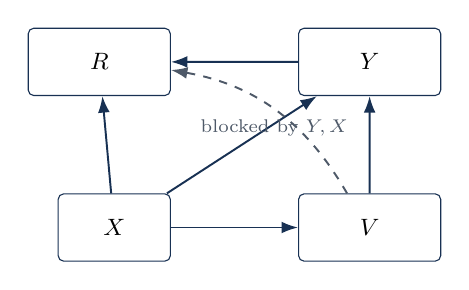
\begin{tikzpicture}[node distance=13mm and 17mm, scale=.95, transform shape]
  \node[box,minimum width=15mm] (u) {$X$};
  \node[box,minimum width=19mm,right=of u] (v) {$V$};
  \node[box,minimum width=19mm,above=of v] (y) {$Y$};
  \node[box,minimum width=19mm,left=of y] (r) {$R$};
  \draw[arr] (v) -- (y);
  \draw[arr] (y) -- (r);
  \draw[arr] (u) -- (v);
  \draw[arr] (u) -- (y);
  \draw[arr] (u) -- (r);
  \draw[darr,bend right=25] (v) to node[note,below] {blocked by $Y,X$} (r);
\end{tikzpicture}
\vspace{4mm}
{\tiny Sources: \textcite{dHaultfoeuille2010,MiaoTchetgen2016}.}
\end{column}
\end{columns}
\end{frame}

% A2 --------------------------------------------------------------------------
\begin{frame}[shrink=7]{付録B：Zhao--Shaoのconditional shadow表現}
常時観測共変量を $X$ とし
\[
\Prb(R=1\mid Y,V,X)=\Prb(R=1\mid Y,X)
\quad\Longleftrightarrow\quad
R\indep V\mid Y,X.
\]
回答者データ上で
\[
\begin{aligned}
f(v\mid y,x,R=1)
&=
\frac{\Prb(R=1\mid v,y,x)f(v\mid y,x)}
{\Prb(R=1\mid y,x)}\\
&=f(v\mid y,x).
\end{aligned}
\]
Bayes則から
\[
f(v\mid y,x)
=
\frac{f(y\mid v,x)f(v\mid x)}
{\int f(y\mid t,x)f(t\mid x)\dd t}.
\]
\begin{alertblock}{本研究との関係}
Zhao--ShaoはGLMパラメータのsemiparametric識別・推定を扱う。
本研究の定理2は，target-specific representerの存在により
平均・裾確率をfull-data lawなしにノンパラメトリックに識別する。
\end{alertblock}
{\tiny Source: \textcite{ZhaoShao2015}.}
\end{frame}

% A3 --------------------------------------------------------------------------
\begin{frame}{付録C：完全ケース版の仮定}
\[
R^{cc}=\1\{\D=\bm1_m\},
\qquad
\pi^{cc}(\Y,\X)=\Prb(R^{cc}=1\mid\Y,\X).
\]
\begin{block}{Complete-case vector missing-IV theorem}
$R^{cc}\indep\V\mid\Y,\X$，$\pi^{cc}>0$，および
\[
\E\{g(\Y,\X)\mid\V,\X\}=0\Rightarrow g(\Y,\X)=0
\]
が成り立つとする。正値関数 $q$ が
\[
\E\left\{\frac{R^{cc}}{q(\Y,\X)}\middle|\V,\X\right\}=1
\]
を満たす正値関数 $q$ を考える。
\end{block}
\end{frame}

\begin{frame}{付録C：完全ケース版の結論と適用範囲}
\begin{block}{一意性}
前頁の仮定の下で
\[
q(\Y,\X)=\pi^{cc}(\Y,\X)\quad\text{a.s.}
\]
であり，完全ケース選択確率と full-data law が識別される。
\end{block}
\begin{alertblock}{適用範囲}
この結果は $\Prb(R^{cc}=1)>0$ の場合のbenchmarkである。
exact top-$K<m$ では $R^{cc}=0$ a.s. なので本文の定理2へ置き換える必要がある。
\end{alertblock}
\end{frame}

% A4 --------------------------------------------------------------------------
\begin{frame}[shrink=6]{付録D：完全ケース版の一意性証明}
真の $\pi^{cc}$ と候補解 $q$ に対し
\[
g(\Y,\X)=\frac{\pi^{cc}(\Y,\X)}{q(\Y,\X)}-1
\]
と置く。すると
\[
\begin{aligned}
0
&=\E\left[R^{cc}\left\{\frac1q-\frac1{\pi^{cc}}\right\}
\middle|\V,\X\right]\\
&=\E\left[\pi^{cc}\left\{\frac1q-\frac1{\pi^{cc}}\right\}
\middle|\V,\X\right]\\
&=\E\{g(\Y,\X)\mid\V,\X\}.
\end{aligned}
\]
$g\ge-1$ で，モーメント条件から $\E(\pi^{cc}/q)=1$，したがって
\[
\E|g|\le2.
\]
$\mathcal B$-completenessにより $g=0$ a.s.，すなわち $q=\pi^{cc}$。
\end{frame}

% A5 --------------------------------------------------------------------------
\begin{frame}{付録E：分布全体の識別には強い仮定を置く}
supported block $S$ について
\[
\pi_S(\Y_S,\mathcal C_S)
=\Prb(R_S=1\mid\Y_S,\mathcal C_S)
\]
とする。
\begin{block}{仮定 B1--B3}
\scriptsize
\[
\text{B1: }\pi_S(\Y_S,\mathcal C_S)>0\quad\text{a.s.},
\]
\[
\text{B2: }R_S\indep\V_S\mid\Y_S,\mathcal C_S,
\]
任意の下有界・可積分な $a$ について
\[
\text{B3: }\E\{a(\Y_S,\mathcal C_S)\mid\V_S,\mathcal C_S\}=0
\Rightarrow a(\Y_S,\mathcal C_S)=0.
\]
\end{block}
\begin{alertblock}{本文との違い}
本文のrepresenter bridgeは一つの $\tau$ に対する解の存在だけを要求する。
B3は全ての関数を分離する完備性であり，full-law識別のための強い条件である。
\end{alertblock}
\end{frame}

\begin{frame}[shrink=6]{付録E：inverse-selection bridgeによるfull-law識別}
\begin{alertblock}{Inverse-selection bridge}
\scriptsize
\[
\omega_S(\Y_S,\mathcal C_S)=\frac1{\pi_S(\Y_S,\mathcal C_S)},
\qquad
\E\{R_S\omega_S(\Y_S,\mathcal C_S)\mid\V_S,\mathcal C_S\}=1.
\tag{ISB}
\]
B1--B3の下で $\omega_S$ は (ISB) の唯一の正値解である。したがって
\[
\E h(\Y_S,\V_S,\mathcal C_S)
=\E\{R_S\omega_S(\Y_S,\mathcal C_S)
h(\Y_S,\V_S,\mathcal C_S)\}
\tag{BR}
\]
によりsupported-block lawがノンパラメトリックに識別される。
\end{alertblock}
\begin{block}{二つのbridgeを区別する}
\scriptsize
representer bridge：target-specific，存在のみ，一意性不要。\par
inverse-selection bridge：full law，一意性と完備性が必要。
\end{block}
\end{frame}

\begin{frame}[shrink=6]{付録E：supported-block定理の証明}
真の $\pi_S$ はB2から
\[
\E\left\{\frac{R_S}{\pi_S(\Y_S,\mathcal C_S)}
\middle|\Y_S,\V_S,\mathcal C_S\right\}=1
\]
を満たす。候補解 $q_S$ に対し
\[
g_S(\Y_S,\mathcal C_S)
=\frac{\pi_S(\Y_S,\mathcal C_S)}{q_S(\Y_S,\mathcal C_S)}-1
\]
と置くと
\[
\E\{g_S(\Y_S,\mathcal C_S)\mid\V_S,\mathcal C_S\}=0.
\]
$g_S\ge-1$，$\E|g_S|\le2$ なのでB3により $g_S=0$ a.s.，よって $q_S=\pi_S$。
さらに反復期待値から
\[
\begin{aligned}
&\E\left[
\frac{R_S}{\pi_S(\Y_S,\mathcal C_S)}h(\Y_S,\V_S,\mathcal C_S)
\middle|\Y_S,\V_S,\mathcal C_S
\right]\\
&\qquad=h(\Y_S,\V_S,\mathcal C_S),
\end{aligned}
\]
したがって回復式 (BR) が従う。
\end{frame}

% A6 --------------------------------------------------------------------------
\begin{frame}[shrink=7]{付録F：有限サポートの完備性はrank条件になる}
$\Y_S$ の条件付きサポートを $\{y_1,\ldots,y_s\}$，
$\V_S$ のサポートを $\{v_1,\ldots,v_t\}$ とする。
\[
M_S(c)=
\left[
\Prb(\Y_S=y_a\mid\V_S=v_b,\mathcal C_S=c)
\right]_{b=1,\ldots,t;\ a=1,\ldots,s}.
\]
\begin{block}{有限サポート条件}
\[
\rank M_S(c)=s\quad\text{a.e. }c
\]
なら
\[
\E\{a(\Y_S,c)\mid\V_S,c\}=0\Rightarrow a(\Y_S,c)=0.
\]
\end{block}
\begin{alertblock}{Weak-but-manyの意味}
単一信号では $\rank M_S<s$ でも，異質な複数信号を組み合わせた
$\V_S^{(L)}$ により行数と分離能力が増え，full column rankを満たし得る。
ただし相互に同じ情報の複製ならrankは増えない。
\end{alertblock}
\end{frame}

% A7 --------------------------------------------------------------------------
\begin{frame}{付録G：self-censoringの支持条件まで比較する}
\begin{block}{Self-censoring}
\scriptsize
\[
D_j\indep\Y_{-j}\mid(\X,Y_j,\D_{-j}).
\]
さらに supported pattern set $\mathcal R$ について
\[
p(d\mid x,y)>c>0\quad(d\in\mathcal R),
\]
\[
d\in\mathcal R,\ d\le d'\quad\Longrightarrow\quad d'\in\mathcal R.
\]
最後の upward closure により，supported patternから観測項目を追加したpatternも必要になる。
\end{block}
{\tiny Source: \textcite{LiMiaoShpitserTchetgen2023}.}
\end{frame}

\begin{frame}{付録G：exact top-$K$ の支持集合との相違}
\begin{block}{Exact top-$K$}
\scriptsize
\[
\mathcal D_{m,K}=\{d:\sum_jd_j=K\}.
\]
$d\in\mathcal D_{m,K}$ に対し $d'>d$ なら $\sum_jd'_j>K$ なので
$d'\notin\mathcal D_{m,K}$。したがって upward closure は成立しない。
\end{block}
\begin{alertblock}{相違はconditional independenceだけではない}
top-$K$ と既存モデルの相違は，censor relationに加え，
positivity，complete-case support，pattern supportの幾何にある。
\end{alertblock}
\end{frame}

% A8 --------------------------------------------------------------------------
\begin{frame}{付録H：個人内ランダム選択帰無}
各人のtail件数を
\[
M_i=\sum_{j=1}^{m}\1(Y_{ij}\in\{1,5\})
\]
とする。公開集合が評価と独立な一様選択なら
\[
\D_i\mid\Y_i,K_i
\sim\Unif(\mathcal D_{m,K_i}).
\]
公開tail件数
\[
S_i=\sum_{j=1}^{m}D_{ij}\1(Y_{ij}\in\{1,5\})
\]
は
\[
S_i\mid M_i,K_i
\sim\operatorname{Hypergeometric}(m,M_i,K_i).
\]
\end{frame}

\begin{frame}{付録H：帰無分布のモーメントとexact test}
\[
\E_0(S_i\mid M_i,K_i)=K_i\frac{M_i}{m},
\]
\[
\Var_0(S_i\mid M_i,K_i)
=K_i\frac{M_i}{m}\left(1-\frac{M_i}{m}\right)
\frac{m-K_i}{m-1}.
\]
$m=10,K=3$ なら $\binom{10}{3}=120$ 通りを個人ごとに列挙できる。
\end{frame}

% A9 --------------------------------------------------------------------------
\begin{frame}{付録I：Model 2は単調性による部分識別である}
過去利用変数 $V_{ij}$ が現在評価を固定しても公開に直接影響することを許し，
順序 $v'\succeq v$ に対して
\[
\pi_j(y,v',c)\ge\pi_j(y,v,c)
\tag{M2-MON}
\]
のみを置く。観測データ法則を $P_O$ とする。
\begin{block}{ノンパラメトリック候補集合}
\scriptsize
\[
\mathcal P_{M2}(P_O)
=\{P:P\mapsto P_O,\ \pi_j>0,\ \text{(M2-MON) holds}\},
\]
\[
\Theta_h^{M2}(P_O)
=\{\E_Ph(Y_j):P\in\mathcal P_{M2}(P_O)\}.
\]
\end{block}
\begin{alertblock}{識別主張}
単調性だけでは $\Theta_h^{M2}(P_O)$ は一般に一点にならない。
Model 2の対象は点推定ではなく，部分識別集合と感度分析である。
\end{alertblock}
\end{frame}

\begin{frame}{付録I：有限サポートのboundsを計算する}
\begin{alertblock}{有限サポートのidentified set}
$Y_j,V_{ij},C_{ij}$ が有限サポートなら
\[
\underline\theta_h
=\inf_{P\in\mathcal P_{M2}(P_O)}\E_Ph(Y_j),
\qquad
\overline\theta_h
=\sup_{P\in\mathcal P_{M2}(P_O)}\E_Ph(Y_j).
\]
閉性・コンパクト性と端点の実現可能性を別途示した場合に限り，min/maxで達成されるsharp boundsと呼ぶ。
\end{alertblock}
\begin{block}{本文に置かない理由}
本文の主結果はtarget-specific point identificationである。
Model 2はexclusion違反に対する頑健性・感度分析として位置づける。
\end{block}
\end{frame}

% A10 -------------------------------------------------------------------------
\begin{frame}{付録J：Model 3はweak-but-many signalsを用いる}
項目 $j$ に対して常時観測される事前信号を
\[
\V_{ij}^{(L)}=(V_{ij1},\ldots,V_{ijL})'
\]
とする。各信号が弱くても，ベクトルとして
\[
D_{ij}\indep\V_{ij}^{(L)}\mid Y_{ij},C_{ij}
\tag{M3-SV}
\]
を満たし，対象 $\tau$ について
\[
\tau(\cdot,c)\in\Range(T_{j,L}^*)
\tag{M3-R}
\]
なら本文のrepresenter bridgeを適用できる。
\begin{alertblock}{必要なのは共同の分離能力}
単一信号の第一段階が弱くても，異質な信号が $Y_j$ の対象方向を共同で分離すればよい。
予測精度や信号数だけではbridge存在は保証されない。
\end{alertblock}
\end{frame}

\begin{frame}{付録J：有限サポートではrankとrangeを区別する}
\begin{block}{Target-specific condition}
$Y_j$ のサポート数を $s$ とし
\[
H_L(c)=
\left[
\Prb(\V_j^{(L)}=v_b\mid D_j=1,Y_j=y_a,C_j=c)
\right]_{a,b}.
\]
\[
\bm\tau(c)\in\Range\{H_L(c)\}
\quad\Longrightarrow\quad
\text{target-specific bridge exists}.
\]
全ての $\tau$ を扱う十分条件は $\rank H_L(c)=s$ である。
\end{block}
\begin{alertblock}{集約時の注意}
$F_{ij}^{pre}=T_L(\V_{ij}^{(L)})$ に集約する場合も，
$\bm\tau(c)\in\Range\{H_F(c)\}$ を別途確認する必要がある。
weak-but-manyは自動的にcompletenessやbridge存在を保証しない。
\end{alertblock}
\end{frame}

\end{document}
